%% General definitions
\documentclass{article} %% Determines the general format.
\usepackage{a4wide} %% paper size: A4.
\usepackage[utf8]{inputenc} %% This file is written in UTF-8.
%% Some editors on Windows cannot save files in UTF-8.
%% If there is a problem with special characters not showing up
%% correctly, try switching "utf8" to "latin1" (ISO 8859-1).
\usepackage[T1]{fontenc} %% Format of hte resulting PDF file.
\usepackage{fancyhdr} %% Package to create a header on each page.
\usepackage{lastpage} %% Used for "Page X of Y" in the header.
\usepackage{ulem} %% Wavey underline
											%% For this to work, you have to call pdflatex twice.
\usepackage{enumerate} %% Used to change the style of enumerations (see below).

\usepackage{amssymb} %% Definitions for math symbols.
\usepackage{amsmath} %% Definitions for math symbols.
\usepackage{amsthm}
\usepackage{braket}
\usepackage{graphicx}
\usepackage{float}
\usepackage{hyperref}

\usepackage{tikz}  %% Pagacke to create graphics (graphs, automata, etc.)
\usetikzlibrary{automata} %% Tikz library to draw automata
\usetikzlibrary{arrows}   %% Tikz library for nicer arrow heads


%% Left side of header
\lhead{\course\\\semester\\Exercise \homeworkNumber}
%% Right side of header
\rhead{\authorname\\Page \thepage\ of \pageref{LastPage}}
%% Height of header
\usepackage[headheight=36pt]{geometry}
%% Page style that uses the header
\pagestyle{fancy}

\newcommand{\authorname}{Nico Bachmann\\Ruben Hutter}
\newcommand{\semester}{Fall Semester 2023}
\newcommand{\course}{Introduction to Databases}
\newcommand{\homeworkNumber}{3}


\begin{document}

\section*{Exercise \homeworkNumber.1}

(practical part)

\section*{Exercise \homeworkNumber.2}

\noindent
Entities:
\begin{enumerate}[-]
\item Supplier(\underline{SName})
\item Company(\underline{CName})
\item Department(\underline{DName}, \uwave{ENo} Budget, \uwave{CName})
\item HeadOfDepartment(\underline{\uwave{ENo}}, \uwave{DName}, Bonus) (Vertical partitioning) or Head of Departement(\underline{ENo}, EName, ESalary, Bonus) (Horizontal partitioning)
\item Employee(\underline{ENo}, EName, ESalary, \uwave{DName})
\end{enumerate}

\noindent
Relations:
\begin{enumerate}[-]
\item has(\underline{\uwave{SName}, \uwave{CName}})
\item affiliated(\underline{\uwave{PCName}, \uwave{SCName}}, Percentage)
\item leads(), owns() and works() "is not needed" after merging their respective relations.

\end{enumerate}

\section*{Exercise \homeworkNumber.3}

\begin{center}
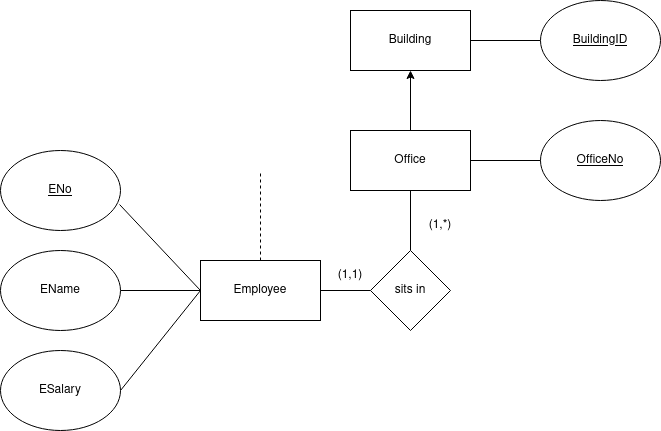
\includegraphics[width=0.65\textwidth]{sheet_3_ex_3.drawio.png}
\end{center}
\begin{enumerate}[-]
\item Employee(\underline{ENo}, \uwave{OfficeNo, BuildingID}, EName, ESalary, \uwave{DName})

\item Building(\underline{BuildingID})
\item Office(\underline{OfficeNo, \uwave{BuildingID}})
\end{enumerate}


\end{document}
